\chapter{Introduction}

Wikipedia defines gamification is the use of game play mechanics for non-game applications, particularly consumer-oriented web and mobile sites, in order to encourage people to adopt the applications. 

The term is almost not exists until in February 2010, as part of the DICE conference, Game designer and professor from Carnegie Mellon, Jesse Schell gave a presentation about a possible future where games, or elements of games, is and will invade every part of our daily live [ref]. The term becomes prominent as several recent books such as Gabe Zicherman's "Game Based Marketing"[ref], who advocated the use of game mechanics in marketing as a form of loyalty program, and Jane Mcgonical's "Reality is Broken"[ref], who assures us that games will make us better and  a solution to the broken reality, and Baron Reeves's "Total Engagement"[ref], who elaborates  games and virtual world will change the way people work and business compete. In the  SXSW 2011, Google backed startup SCVNGR CEO Seth Priebatsch talks[ref] about game is the new layer that similar to the social layer, "will change the world".  

In IT industry research, Gartner [ref1] predicts that by 2015, more than half of companies managing innovation processes will employ Gamification, a process of applying game mechanics to non-game contexts. In that same time frame, M2 Research [ref2] forecasts that the game mechanics production will generate 1.6 billion in revenues and will account for 23 percent  of social media marketing budgets. 

In the newly release Gartner Hype Cycle report, gamification, along with big data and internet of things, are added to the 2011 hype cycle, that weren't present in 2010. According to Gartner, currently gamification is on the rise to the peak of the hype, the stage of the "peak of inflated expectation", with 5-10 years of mainstream adoption. [see figure 1.1]. 

\begin{figure}[htbp]
	\centering
		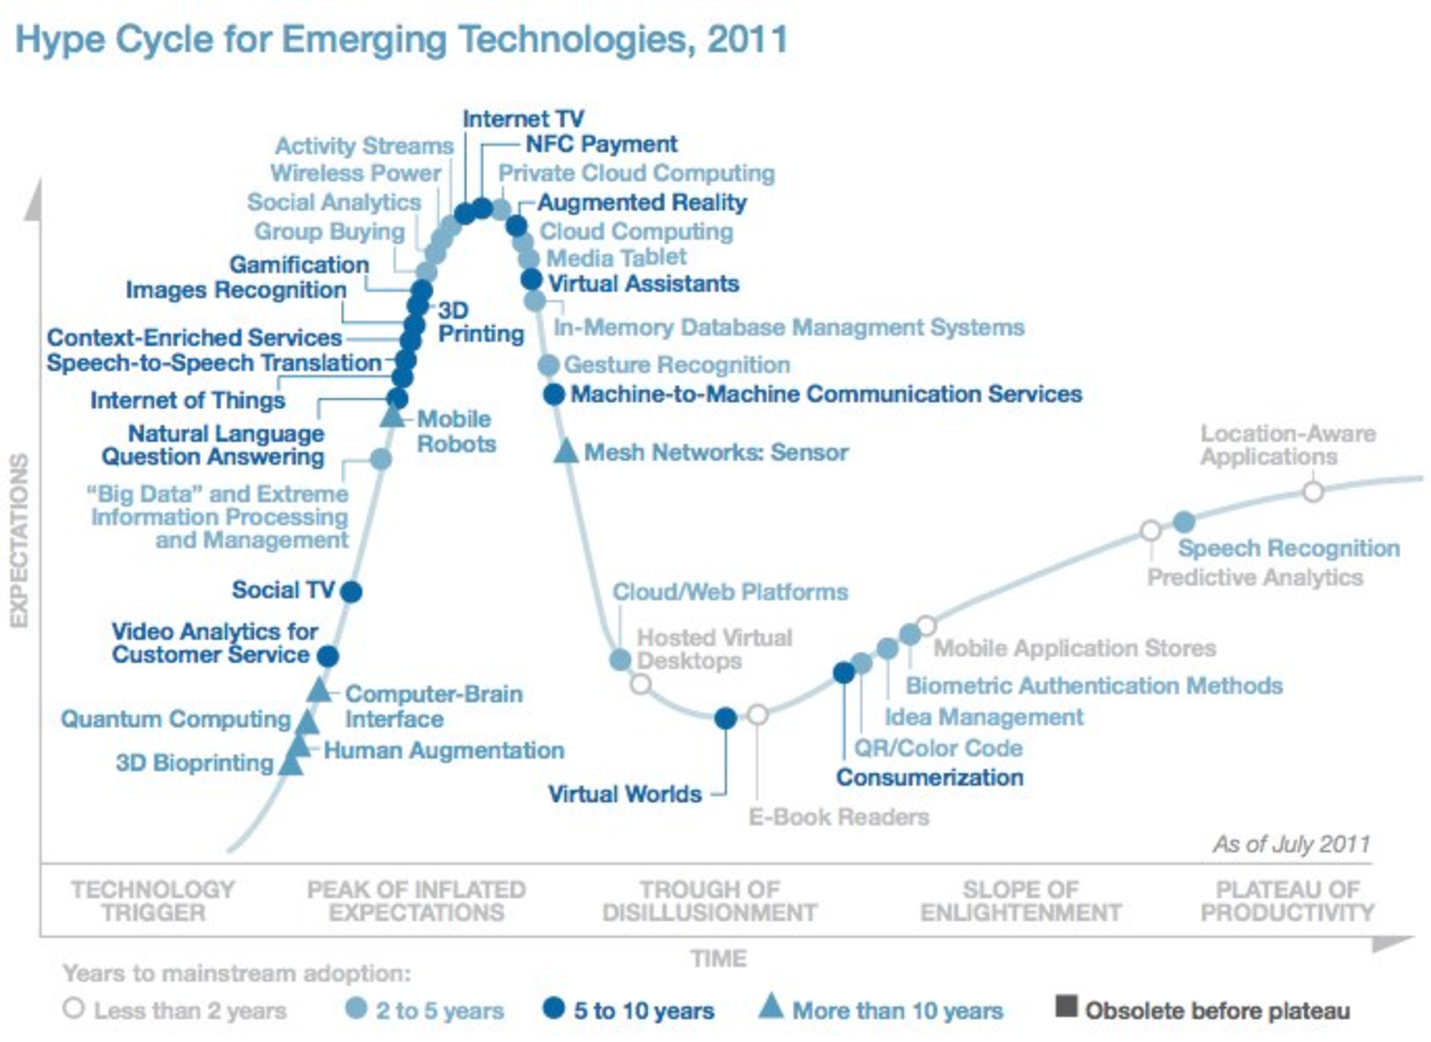
\includegraphics[scale=0.7]{gartner-hype-cycle.pdf}
		\caption{2011 Gartner Hype Cycle}
		\label{fig:Gartner-2011-Hype-Cycle}
\end{figure}

Gartner use the hype cycle theory to track technology adoption, after the peak period, the technology will slip into the trough of disillusionment and some technologies will start climbing the slope of enlightenment and eventually reach the plateau of productivity.  As any technology, Gamification will inevitably slip into the disillusionment trough where the hype is passed and the mass realize there are a lot of unsolved and criticism will arrive. The question remains if gamification will eventually climb out of the trough and appear in the plateau of the cycle.

In fact, there are already quite a lot critique of gamification in the media. Some called it a merely buzzword, a hype-up version of mileage loyalty program, or a superficial "pointification", where often misses element such as storytelling and experiences which are central to what make games effective.[ref]

More and more game designers and researchers are looking into the deeper practice of gamification. Amy Jo Kim presents Smart Gamification which focus on designing the effective Player Journey with intrinsic preferred over extrinsic reward.[ref] Jane Mcgonical is emphasizing the aspect of "Playfulness" in an gamification instead of game mechanics.[ref]. Similarly, In his popular google tech talk, researcher Sebastian Deterding criticized the current practice of simple gamification and stress the important of "meaningful play".[ref]

It is surely becoming an IT phenomenon where gamification lie in between a layer that will change the world and a meaningless buzzword".

The goal of this paper is to review the gamification technique in a scientific way, examine most of the commonly employed game mechanics with their usages, effectiveness. 
